\documentclass[oneside,11pt]{amsart}
\usepackage[utf8]{inputenc}%
\usepackage[english]{babel}%
\usepackage{amsmath,amssymb,amsthm,amsfonts}%
\usepackage[unicode]{hyperref}%
\usepackage{mathrsfs,bbm}%
\usepackage{paralist}
\usepackage{color}
\usepackage{longtable}
\usepackage{array}
\newcolumntype{L}[1]{>{\small\raggedright\arraybackslash}m{#1}}
\newcolumntype{T}[1]{>{\footnotesize\raggedright\arraybackslash}m{#1}}
\usepackage{stmaryrd}%
%\usepackage{refcheck}
\usepackage{graphicx}
\usepackage[DIV15]{typearea}
\usepackage{multicol,tikz}
\usepackage{datetime}
\usepackage{cleveref}

\usepackage[shadow]{todonotes}

\usepackage{etoolbox}
\patchcmd{\section}{\scshape}{\Large\itshape\bfseries}{}{}

\usepackage{caption}
\captionsetup{labelformat=empty,labelsep=none}

\hypersetup{
  colorlinks=true,
  linkcolor=blue!50!red,
  urlcolor=green!60!black
}

%%%%%%%%%%%%%%%%%%%%%%%%%%%%%%%%%%%%%%%%%%%%%%%%%%%%%%%%%%%%%%%%%%%%%%%%%%%%%%%%%%%%%%%%
\synctex=1
%%%%%%%%%%%%%%%%%%%%%%%%%%%%%%%%%%%%%%%%%%%%%%%%%%%%%%%%%%%%%%%%%%%%%%%%%%%%%%%%%%%%%%%%
%%%%%%%%%%%%%%%%%%%%%%%%%%%%%%%%%%%%%%%%%%%%%%%%%%%%%%%%%%%%%%%%%%%%%%%%%%%%%%%%%%%%%%%%
\newcommand{\score}[1]{\textit{#1}\addtocounter{totalscore}{#1}}
\newcommand{\razdel}[1]{\smallskip\underline{\textbf{#1:}}\smallskip}

\newcommand{\note}[1]{{\sf{}\color{blue}(#1)}}

\begin{document}

\title[MATH 3100: INTRODUCTION TO PROBABILITY]{MATH 3100: INTRODUCTION TO PROBABILITY}
\author{Leonid Petrov\\Fall 2023\\Sections 001 and 002}
\date{Compiled on \today, \currenttime.\\An up to date syllabus is always on \texttt{GitHub} at \url{https://github.com/lenis2000/Syllabi/blob/master/Syllabus_3100_f23.pdf}. For direct PDF download, use \href{https://github.com/lenis2000/Syllabi/raw/master/Syllabus_3100_f23.pdf}{\texttt{this link}}.
	\LaTeX{} source with \textit{changes} to the syllabus is \href{https://github.com/lenis2000/Syllabi/blob/master/Syllabus_3100_f23.tex}{\texttt{here}}
(click ``History'').}
\maketitle

\bigskip


\section{A mathematical study of randomness}

How random is everything around us, and what chance do we have of understanding it? What to do when unsure, and how to do it right? How many falling stars will you see as you walk outside one beautiful night? 

Probability theory is a mathematical study of uncertainty. It is a rigorous foundation of statistics --- and many areas of human knowledge operate in a language of statistics nowadays (yes, and robots use it, too!). The course introduces fundamental concepts, ideas, and techniques of probability theory. It will provide the foundational mathematical knowledge needed to address the questions above and help you develop intuition about randomness.


\begin{figure}[h]
	\begin{tabular}{ccc}
		
\includegraphics[height=.32\textwidth]{img/Bond_percolation_p_51.png}
		&\hspace{10pt}
\includegraphics[height=.32\textwidth]{img/Amas_de_percolation_gray.png}
		&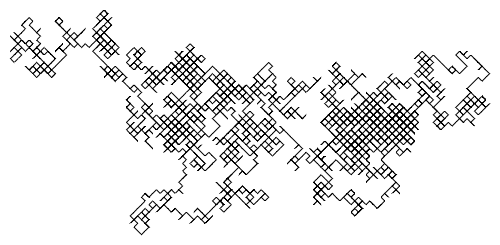
\includegraphics[angle=90,height=.32\textwidth]{img/RW1.png}
	\end{tabular}
	\def\figurename{}
	\caption{Examples of random structures: bond percolation
	\href{https://en.wikipedia.org/wiki/Percolation_theory}{\texttt{close-up}}
	(left),
	at a \href{https://commons.wikimedia.org/wiki/File:Amas_de_percolation.png}{\texttt{larger scale}} (center),
	and
	a 
	\href{https://en.wikipedia.org/wiki/Random_walk\#Lattice_random_walk}{\texttt{random walk}}
	(see also a
	\href{https://upload.wikimedia.org/wikipedia/commons/f/f3/Random_walk_2500_animated.svg}{\texttt{simulation}} 
	of a random walk).
	\emph{Note:
	this PDF has green clickable links, like in the previous sentence.
	This feature only works if you download the PDF first --- it will not work in a browser on GitHub.}
	}
\end{figure}

\subsection*{What you will get from this course}

\begin{enumerate}[\bf{}1.]
	\item Mastery of basic probability concepts:
	\begin{enumerate}[(a)]
		\item What is a probability space and how to translate commonly-sounding problems into this language;
		\item How to count (in an advanced way) to compute probabilities;
		\item What is a random variable, a probability distribution,
		and what are their main quantitative properties;
		\item 
		How commonly encountered probability 
		distributions (binomial, Poisson, exponential, Gaussian) look like and behave,
		what are 
		their properties, and in which situations they typically arise.
	\end{enumerate}

	\item How large random systems behave, and what the 
	bell-shaped curve
	\raisebox{-8pt}{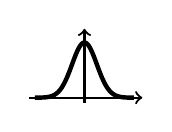
\begin{tikzpicture}
		[scale=.7]
		\draw[ultra thick, domain=-.9:.9] plot[samples=300] ({\x}, {2.7128^(-10*\x*\x)});
		\draw[->, thick] (-1.01,0)--(1.05,0);
		\draw[->, thick] (0,-.1)--(0,1.25);
	\end{tikzpicture}}
	has to do with this.
	\item How to describe and quantify the mutual dependence of random events,
	and how to use such a description 
	to infer properties of ``hidden'' random events.
	\item How to apply probability theory to model real-life processes. For example,
		how to use Bayes theorem to understand various medical tests.
	\item How to collaborate on solving probability problems in pairs, small groups, and online,
	and present solutions clearly and efficiently.
	% \item How to design probability problems (for example, for the
	% final exam), and evaluate problems presented by others.
	\item In what ways probability theory is connected to science, engineering, and other branches of knowledge.
\end{enumerate}

\subsection*{Prerequisite} You should have taken at least one semester of calculus (MATH 1320 level): a mathematical study of random variables often requires single and double integrals and infinite series.

\subsection*{What this course is and what it is not}

This course in probability \emph{theory} belongs to pure mathematics, with rigorous definitions, calculations, and proofs. However, the objects we study are motivated by real-life applications, so pure mathematical arguments often appeal to our common sense understanding of these objects. There will be opportunities to explore (and discover new) connections between the theory studied in the course with the real world.

Also, this course does not thoroughly discuss \emph{applications to statistics}. Probability theory focuses on developing the mathematical side, and statistics apply these mathematical theories to real data (coming from observations). In this course, we will not discuss how to analyze data from observations --- there are courses in statistics for that.

\section{Necessary information}
\label{sec:necc}

\subsection{Meeting times}{\ }\\
\label{sub:meeting_times}


\begin{tabular}{|r|l|l|}
	\hline
	& Section 001 & Section 002 \\
	\hline
	\textbf{Class times} & & \\
	August 23 --- December 4 & MoWe, New Cabell 232 & MoWe, New Cabell 323 \\
	& 5:00PM - 6:15PM & 3:30PM - 4:45PM \\
	\hline
	\textbf{Midterm 1} & September 25, class time & September 25, class time \\
	\hline
	\textbf{Midterm 2} & October 25, class time & October 25, class time \\
	\hline
	\textbf{Final exam} & Friday, December 15  & Tuesday, December 12\\
	& 2:00PM - 5:00PM & 2:00PM - 5:00PM
	\\
	\hline
\end{tabular}

\medskip

\textbf{Note on scheduling the final exams:} Anyone from both sections can use any final exam times. If December 12 works for all, we will have a combined final exam that day in a bigger room. If not, we will have two final exams on December 12 and 15. I will ask you about your preferences in the middle of the semester.


\subsection{Lectures+quizzes on Mondays, and problem solving on Wednesdays}
Typically, on Mondays we focus on introducing new material through lectures, while on Wednesdays, we emphasize problem-solving practice during "discussion" sessions. On Mondays, we also typically have quizzes. See \Cref{sub:schedule} for the schedule.

On Wednesdays, we work as a class and in groups to hone our probabilistic thinking skills, by solving problems from the current weekly problem set. Monday lectures for both sections are recorded, posted on Canvas with notes, and have a "watch by" deadline. Wednesday classes are not recorded. Homework consists of problem sets and catching up with lectures (by watching video or reviewing lecture notes from another section). Problem sets are handed out on Wednesdays (and posted to Canvas), and we start working on them in class.

\textbf{Lectures for two different sections will be different to cover all the necessary material, so watch or review notes for both lectures each week, either in person or in recording.} But do not worry if did not watch a particular lecture --- come to class on Wednesday and catch up during problem solving.



\subsection{Instructor}

Leonid Petrov, Kerchof 209

\textbf{Questions to the instructor:} \href{mailto:leniapetrov+f23@gmail.com}{\texttt{leniapetrov+f23@gmail.com}}

\textbf{Instructor office hours:} 
Mondays 1:30-2:30 pm; Wednesdays 11:30am-12:30pm; and by appointment $\downarrow$

You can automatically schedule an office hours appointment 
at \href{https://lpetrov.cc/teaching/}{\texttt{this page}} (you do not need an appointment for 
regular office hours M1-2, W12-1).
You can make as many appointments as you need throughout the semester.
Each appointment scheduled online
must be made at least 4 hours prior to the time of the appointment.
Office hours by appointment are on zoom (\href{https://virginia.zoom.us/j/97731277583?pwd=UFNvZ0NHNWRRaHpPTGYrTnJiZ3Rpdz09}{\texttt{link}}); 
in-person option is also possible by request (ask about this in a separate email).


\subsection{About the instructor}
I am an Associate Professor in the Department of Mathematics at UVA, and I've
been here since 2014. My research area is probability theory (very appropriate
for this course!). More precisely, I am using exact formulas to study large
random systems. I also like computer simulations of random systems like 
\href{https://d3m0khvr0ybm92.cloudfront.net/img/blog/heart/UVA_colors_small.png}{\texttt{this one}}.
I'm happy to tell you more if you're
interested.


\subsection{Textbook}
\label{sub:main_textbook}

Anderson, Sepp\"al\"ainen, Valk\'o, \emph{Introduction to Probability}, 1st Edition.

ISBN-13: 978-1108415859; 
ISBN-10: 9781108415859.

See also \Cref{success} below for discussion 
of how we'll use the textbook,
and for other helpful resources.

\section{Assessing your learning}

Learning mathematics means \emph{doing} mathematics: during class meetings, on your own, and in groups.
In this course, doing mathematics mainly amounts to solving problems.
The following aspects are assessed in this course:

\subsection{Course engagement (25\%)}

I am putting a lot of emphasis
into the various engagement components which ask you to interact with 
your peers (and the instructor) while learning the material. This includes:

\begin{itemize}
	\item \textbf{In-class participation}. 
		Being present and involved in discussions at most of the in-class meetings
		is essential to getting a hands-on experience 
		in problem solving. 
		I understand that many people cannot participate in all class meetings due to various
		circumstances. 
		I expect to give full credit for class participation 
		if you come to at least 75\% of the class meetings (not counting midterms).
	\item \textbf{Quizzes}. 
		The quizzes are based on the material similar to the previous homework.
		Lowest $1.5$ quiz grades our of 11 total quizzes are dropped.
		See the course schedule (\Cref{sub:schedule}) for quiz dates.
	\item \textbf{Office hours}. Come to office hours (if needed, 
		sign up for appointments, see \Cref{sub:meeting_times}) 
		with questions about the material.
		I am always happy to discuss your ideas and explain math.
		As a rule, I expect every student to come to office hours or schedule a one-on-one appointment
		at least once throughout the semester.
\end{itemize}

I expect most people paying attention to the class, attending class meetings, interacting with peers, and solving most quiz problems will get close to full credit for the course engagement.

\subsection{Problem sets (20\%)}

Problem sets is a graded part of the homework. They are handed out on Wednesdays (and posted to Canvas).
We start working on them in class.

\medskip

\begin{enumerate}[$\bullet$]
	\item Weekly problem sets consist of textbook and other problems aligned with 
		lectures and 
		in-class discussions, to
		help you practice new concepts and techniques. 
		The written solutions are typically due on
		Tuesdays at 10pm, and sometimes on Thursdays (see the schedule in \Cref{sub:schedule}).
	\item You are encouraged to work together on problem sets in class and outside of class.
		Group work allows you to 
		take advantage of challenge-defend discussions, which help understand things
		better.
		However, each student needs to submit her/his own written work, 
		and should write this up individually. 
		This helps better retain the material and prepare for tests.
	\item 
		When solving homework problems, use your math and common sense understanding to check for your own mistakes,
		see \Cref{sub:problem_solving} for details.
	\item 
		The work \emph{must be submitted only on Canvas} --- 
		take pictures or scan your work, ensure it is readable, put it into a \emph{single PDF file with correct orientation}, and upload it to the Canvas assignments before the deadline. Failure to make a single PDF might result in zero points (after a first warning).
\item

The written solutions are graded ``coarsely'', that is,
		each problem set will be assigned one of four grades: 
		\begin{equation*}
			\begin{tabular}{l|l|l|l|l}
				Grade & VG (very good) & G (good) & OK   & N \\
				\hline
				& \parbox{.21\textwidth}{All problems solved correctly with minor issues like arithmetic mistakes, and solutions explained
				in full detail}
				& \parbox{.21\textwidth}{Most problems solved correctly, and solutions explained in reasonable (close to full) detail}
				& \parbox{.21\textwidth}{ {\ }\\More than $3/4$ of problems attempted, many 
				solutions are incorrect, incomplete, or not explained in detail, 
				but the work displays adequate understanding of most of the material\\{}}
				& \parbox{.21\textwidth}{Work not submitted on time, or less than $3/4$ of problems 
				attempted, or most solutions are incomplete, or work clearly displays lack of understanding of most of the material}\\
				\hline
				\%    & 100\%          & 90\%     & 75\% & 0\%
			\end{tabular}
		\end{equation*}
		It is expected that most students 
		who put reasonable effort into the work
		will get VG or G grades. 
\end{enumerate}

\subsection{Midterm tests (2 tests each worth 15\%; 30\% in total)}

There are two midterm tests
held
during regular class times, on \textbf{September 25} and \textbf{October 25}.
They have
similar taste as homework and quizzes, and test basic knowledge of the material.

\textbf{Formula sheet}.
A two-sided letter-size formula sheet, hand-written by yourself, is allowed on each midterm test and on the final exam. Preparing this formula sheet will help you review the material and paint a systematic picture of the material in your mind. In general, formula sheets cannot contain any photocopied or printed material --- do everything by hand (of course, you can include any theorems, formulas, pictures, examples, etc). One exclusion: if you write the formula sheet out on a tablet and print, this is allowed, if helps --- but don't copy formula sheets from other people.

I encourage you to collaborate on preparing for the tests, but needless to say that each student must work individually during the test and the final exam.
When solving midterm problems, use your math and common sense understanding to check for your own mistakes,
see \Cref{sub:problem_solving} for details.


\subsection{Final exam (25\%)}

The final exam will be cumulative but will put more focus on topics covered after the second midterm. A formula sheet is also allowed, the same format as for midterms. Use your math and common sense understanding on the final exam to check for mistakes (see \Cref{sub:problem_solving}).


\subsection*{Letter grades}

The scale by which course percent grades are turned into course letter grades
will most likely be the following:
\begin{equation*}
	\begin{tabular}{l|l|l|l|l|l|l|l|l|l|l|l|l|}
		Grade      & $ A+	$ & $A	$ & $A-	$ & $B+	$ & $B	$ & $B-	$ & $C+	$ & $C	$ & $C-	$ & $D+	$ & $D	$ & $D-$ \\
		\hline
		Minimum \% & 100     & 93   & 89    & 86    & 82    & 79    & 76    & 72    & 69    & 66    & 62    & 59
	\end{tabular}
\end{equation*}
I reserve the right to slightly change this grade scale after the
final exam.
This may be needed
to better incorporate into the letter grade
possible fluctuations in the difficulty level of 
midterms and the final.

\section{How to succeed in the course}
\label{success}

If you have read the long syllabus through here, you are on the right
track to succeed!

\subsection{General things}

The best way to learn in the course is to 
come to all classes, read the textbook,
and do all the homework problems on your own or in collaboration.
This will prepare you well for quizzes and tests.

\subsection{Main textbook}

The textbook \emph{Introduction to Probability} by Anderson, Sepp\"al\"ainen, and Valk\'o 
is 
an excellent resource 
to gain understanding of the course material. Some notes about it:

\begin{enumerate}[$\bullet$]
	\item I strongly encourage you to read the textbook in parallel with 
		the lectures, as lectures are largely based on the textbook.
		The textbook includes many examples and
		extra exercises which augment the concepts discussed in class.
	\item The textbook contains much more material than will be covered in classes, so it
		makes sense to come to classes to note which parts are omitted
		(and so won't be in tests and quizzes).
\end{enumerate}

\subsection{Additional textbooks}

\begin{enumerate}[$\bullet$]
	\item 
		\emph{``Probability'' by Jim Pitman} is a reasonable alternative textbook.
	\item 
		\emph{Free textbook} 
		\emph{``Introduction to Probability'' by Grinstead and Snell}.
			Download: \url{https://math.dartmouth.edu/~prob/prob/prob.pdf};
			Accompanying web page: \url{https://www.dartmouth.edu/~chance/teaching_aids/books_articles/probability_book/book.html}.
\end{enumerate}

These textbooks contain additional problems and material.
They may be helpful if you want a deeper understanding of
some concepts, or if you want to read an exposition of the
familial material in a different style, which might be very
helpful for better learning.

(It absolutely not required that you buy or read these books.)

\begin{enumerate}[$\bullet$]
	\item Free video course on Probability by R.~Vershynin:
	\href{https://www.math.uci.edu/~rvershyn/teaching/ugp/ugp.html}{\texttt{link}}
\end{enumerate}

\subsection{Problem solving and self-checking}
\label{sub:problem_solving}

Solving problems, one can easily make arithmetic mistakes,
and this is understandable. However, 
we are doing probability theory, so some answers to problems
may be easily dismissed as wrong
based on common sense. 
The most obvious examples are 
getting a \emph{negative probability}; \emph{probability strictly greater than 1};
getting a \emph{negative variance}; and so on.
It is expected that you use this type of common sense to filter out 
such ``obviously wrong'' answers.
Solid partial credit will be given even in the case when you get an ``obviously
wrong'' answer, and note near it:
\begin{quote}
	``Well, this answer is clearly incorrect because $\{\textnormal{expanation}\}$''.
\end{quote}
``Obviously wrong'' answers without such a note 
will result in much less partial credit for the whole problem.

\subsection{Extra reading}

The popular book
\emph{``How Not to Be Wrong: The Power of Mathematical Thinking'' by Jordan Ellenberg}
discusses how math touches every aspect of real life, and has 
numerous examples related to probability and statistics. 
I can recommend this nice book as a parallel reading. Some
examples I learned from this book might be mentioned in class.
(It absolutely not required that you buy or read this book.)

\subsection{Office hours}

I am available during office hours to answer questions on the content of the 
course, clarify various points, and I can also help you with problem sets. 
Besides regular office hours, you can schedule appointments online, see 
\Cref{sec:necc}.

\subsection{Math Collaborative Learning Center}

The Math Department 
Collaborative Learning Center
is available for helping students in this course: 
see \url{https://math.virginia.edu/undergraduate/MCLC/}
for more information and schedule. 
(Usually it takes a week or so after the semester starts for MCLC to start working.)

\subsection{Other resources}

There is a number of online resources which may help you while doing the homework problems:
Khan Academy, Wikipedia, and many other 
places contain lots of basic material on probability theory. Google Search
in general
is also a valuable resource.

\subsection{Collaboration}
\label{collaboration}

Group work on problem sets is allowed and strongly encouraged during Wednesday classes.
Discussions are in general very helpful and inspiring. When completing the written homework assignments, everyone must write up his or her own
solutions in their own words, and cite any reference 
(other than the textbook and
class notes) that you use. Quotations and citations are part of the Honor Code for both UVa
and the whole academic community. 

It is very important that you truly understand the homework solutions you hand
in, otherwise you may be unpleasantly surprised by your quiz and test results.

\section{Course schedule}
\label{sub:schedule}

% \noindent Add/drop information: \href{https://registrar.virginia.edu/enrollment-information/fall-enrollment-2023}{\texttt{see here}}.
\bigskip

\begin{quote}
	The course has 3 ``pillars'': central limit theorem for Gaussian approximation, 
	Poisson processes, and conditional expectations. 
	Plus there are several technical things to learn: random variables, expectations as integrals, 
	joint distributions, etc.
\end{quote}

\bigskip

All sections are from the main textbook (see \Cref{sub:main_textbook}).

\medskip

\begin{enumerate}[\bf{}{[}week 1{]}]
	\item 8/23.
		Introduction. Sample space, axioms of probability, random sampling, review of counting,
		infinitely many outcomes.
		(\texttt{1.1-1.3}).
	\item 8/28[Q1], 8/30.
		No problem set due.
		Hypergeometric sampling. Infinitely many outcomes. Geometric series. 
		Rules of probability, Venn diagrams. Random variables (first look). 
		(\texttt{1.3-1.5}).
	\item 9/4[Q2], 9/6.
		\emph{PS1} due on Tuesday at 10pm.
		Conditional probability, Bayes' formula, independence.
		(\texttt{2.1-2.3}).
	\item 9/11[Q3], 9/13.
		\emph{PS2} due on Tuesday at 10pm.
		Independent trials, birthday problem, conditional independence, 
		probability distribution of a random variable
		(\texttt{2.4-2.5, 3.1}).
	\item 9/18[Q4], 9/20.
		\emph{PS3} due on Tuesday at 10pm.
		Probability distribution of a random variable,
		cumulative distribution function, expectation, variance, Gaussian distribution (\texttt{3.2-3.5}).
	\item 9/25, 9/27. \textbf{Midterm 1, September 25.}
		No problem set due, practice problems posted a week before the midterm.
		Probability distribution of a random variable,
		cumulative distribution function, expectation, variance, Gaussian distribution (\texttt{3.2-3.5}).
	\item 10/4[Q5].
		\emph{PS4} due on Thursday at 10pm.
		Gaussian distribution, normal approximation,
		law of large numbers,
		applications of normal approximation
		(\texttt{3.5, 4.1-4.3}).
	\item 10/9[Q6], 10/11.
		\emph{PS5} due on Tuesday at 10pm.
		Gaussian distribution, normal approximation,
		law of large numbers,
		applications of normal approximation
		(\texttt{3.5, 4.1-4.3}).
	\item 10/16[Q7], 10/18. 
		\emph{PS6} due on Tuesday at 10pm.
		Poisson approximation, exponential distribution, Poisson process
		(\texttt{4.4-4.6}).
	\item 10/23, 10/25. \textbf{Midterm 2, October 25.}
		No problem set due, practice problems posted a week before the midterm.
		Poisson process, gamma distribution (\texttt{4.6}). 
	\item 10/30[Q8], 11/1.
		\emph{PS7} due on Tuesday at 10pm.
		Joint distributions (\texttt{6.1-6.3}).
		Sums of independent random variables and related topics (survey of 
		selected material of chapters \texttt{7} and \texttt{8}).
	\item 11/6[Q9], 11/8.
		\emph{PS8} due on Tuesday at 10pm.
	\item 11/13[Q10], 11/15.
		\emph{PS9} due on Tuesday at 10pm.
		Law of large numbers, central limit theorem (\texttt{9.1-9.3}).
	\item 11/20.
		\emph{PS10} due on Tuesday at 10pm.
		Conditional distributions
		(\texttt{10.1-10.3}).
	\item 11/27[Q11], 11/29.
		No problem set due.
		Conditional distributions (\texttt{10.1-10.3}).
	\item 12/4.
		\emph{PS11} due on Tuesday at 10pm.
		Repair credit problem set due on Thursday at 10pm.
		Conditional distributions (\texttt{10.1-10.3}),
		final exam practice problems.
\end{enumerate}

\bigskip

[Q$x$] means quiz number $x$ and \emph{PS$y$} means problem set number $y$, where $x,y=1,2,\dots,11$.

\section{Policies}

\subsection{Late/make up work} Each homework
assignment will have due date and time by which it must be submitted to Canvas.
After the 1-hour grace period, late assignments are not accepted.
There will also be no make up for the quizzes or midterm tests.
However, if you have special needs, emergency, or unavoidable conflicts, please
let me know as soon as possible, so we can arrange a workaround for midterms and the final exam.

\subsection{AI generated solutions}

If you are using chatGPT or a similar AI text generating tool for homework problems, please make a note about 
this in the beginning of your solution. These tools are good at writing lots of text, but quite terrible at 
solving problems --- they produce wrong answers about half the time. I am not forbidding the use of such tools, but I will 
look at these solutions with increased scrutiny.

\subsection{Special needs}

All students with special needs requiring accommodations should present the
appropriate paperwork from the Student Disability Access Center (SDAC). It is
the student's responsibility to present this paperwork in a timely fashion and
follow up with the instructor about the accommodations being offered.
Accommodations for midterms or final exams (e.g., extended time) should be arranged at
least 5 days before an exam.

\subsection{Honor Code} The University of Virginia Honor Code applies to this
class and is taken seriously (in particular, 
see \Cref{collaboration} on homework collaboration).
Any honor code violations,
especially in written tests (midterms and the final exam)
will be referred to the
Honor Committee.












\end{document}
